\chapter{Qiitaで数式を書きましょう}
\label{chap:QiitaFormula}
 \begin{center} 
河野悦昌  \textbf{オープンフォース}

 \end{center} 
\section{TeX式を簡単に作成する}
\label{sec:2-1}

https://webdemo.myscript.com/views/math.html\#
ここで数式を手書きで書くとTeX式に直してくれます

\begin{reviewimage}
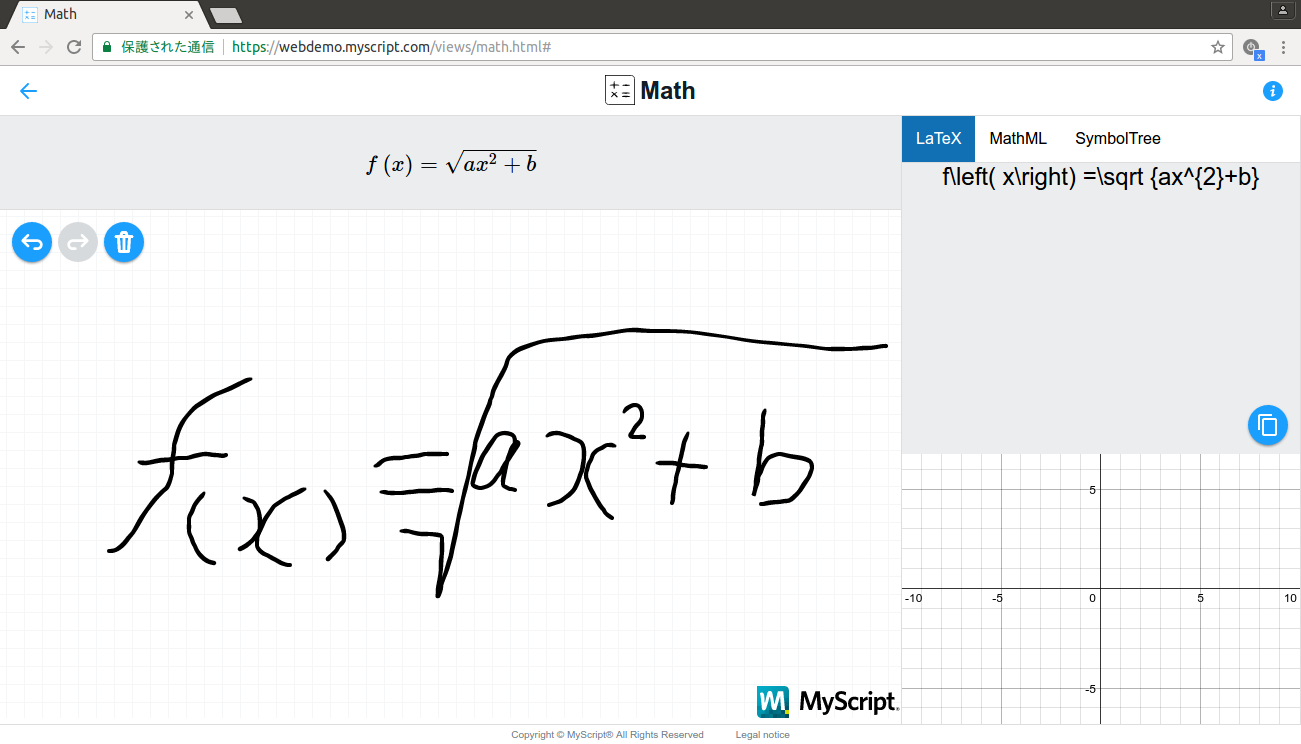
\includegraphics[width=\maxwidth]{./images/f7182c75-f4fe-07a4-6d54-c76f5d514db8.png}
\caption{image}
\label{image:QiitaFormula:f7182c75-f4fe-07a4-6d54-c76f5d514db8}
\end{reviewimage}

\subsection*{Qiitaで書く}
\addcontentsline{toc}{subsection}{Qiitaで書く}
\label{sec:2-1-1}

先のページで作ったLaTeX式をコピーします。

\begin{reviewemlist}
f\reviewbackslash{}left( x\reviewbackslash{}right) =\reviewbackslash{}sqrt \{ax\textasciicircum{}\{2\}+b\}


\end{reviewemlist}

この数式をQiitaで書いてみます。

\begin{quote}
「 TeXで作った式 \textdollar{} f\reviewbackslash{}left( x\reviewbackslash{}right) =\reviewbackslash{}sqrt \{ax\textasciicircum{}\{2\}+b\} \textdollar{} です 」

\end{quote}

と書くと

「 TeXで作った式  $ f\left( x\right) =\sqrt {ax^{2}+b} $  です 」

となります。

ブロック書式で書くには

\begin{quote}
```math

「 TeXで作った式  f\reviewbackslash{}left( x\reviewbackslash{}right) =\reviewbackslash{}sqrt \{ax\textasciicircum{}\{2\}+b\}  です 」

```

\end{quote}

と書くと

\begin{equation*}
「 TeXで作った式  f\left( x\right) =\sqrt {ax^{2}+b}  です 」
\end{equation*}

となります。
